\documentclass[10pt]{article}
\usepackage{longtable}
\usepackage{float}
\usepackage{wrapfig}
\usepackage{rotating}
\usepackage[normalem]{ulem}
\usepackage{amsmath}
\usepackage{textcomp}
\usepackage{marvosym}
\usepackage{wasysym}
\usepackage{amssymb}
\usepackage{hyperref}
\usepackage{color,soul} % for highlighting
\usepackage{graphicx}
\graphicspath{{/Users/benjaminbass/seacloud/class/earthMaterials/picBank/}}

\usepackage{frame,color}
\usepackage{framed}
\usepackage{minibox}

% \usepackage[T1]{fontenc}
% \usepackage{tilting} %bring title up
% \setlength{\droptitle}{-10cm}

\usepackage[version=3]{mhchem}
% How to Use MChem
% \ce{SO4^2-}
% \ce{^{227}_{90}Th+}
% \ce{A\bond{-}B\bond{=}C\bond{#}D}
% \ce{CO2 + C -> 2CO}
% \ce{SO4^2- + Ba^2+ -> BaSO4 v}


\author{Benjamin Bass}
\date{2 March 2016}
\title{\vspace{-2.0cm}Talc} %bring title up temporary Fix

\begin{document}

\maketitle

% \framebox{Use frameboxes until figure out alignmen}

\begin{center}
  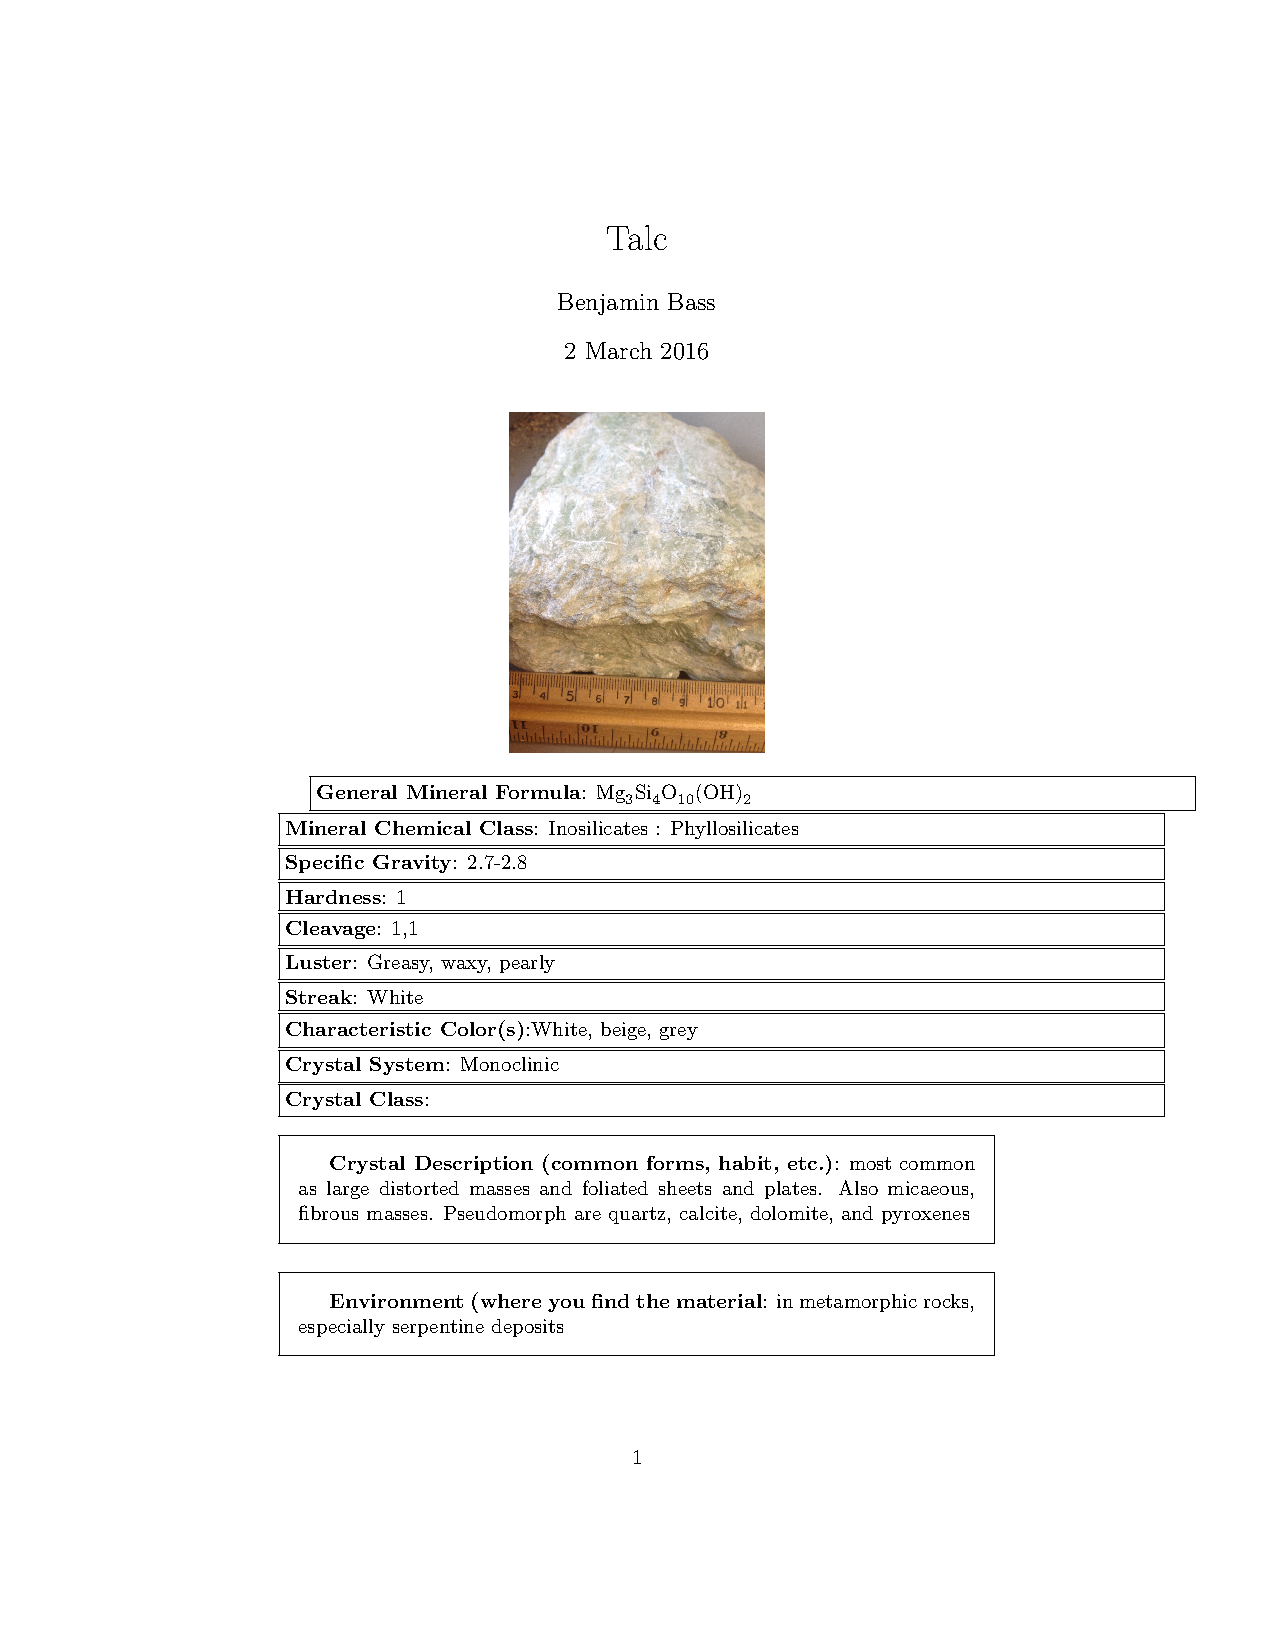
\includegraphics[scale=.05]{talc}\footnote{Soft, greasy, look and feel. White, greenish, pale brown. Often associated with hydrothermal alteration of ultramafic rocks.}
\end{center}



\framebox[15cm][l]{\textbf{General Mineral Formula}: \ce{Mg3Si4O10(OH)2} }\
\framebox[15cm][l]{\textbf{Mineral Chemical Class}: Inosilicates : Phyllosilicates }\
\framebox[15cm][l]{\textbf{Specific Gravity}: 2.7-2.8 }\
\framebox[15cm][l]{\textbf{Hardness}: \hl{1} }\
\framebox[15cm][l]{\textbf{Cleavage}: 1,1 Perfect }\
\framebox[15cm][l]{\textbf{Luster}: Greasy, waxy, pearly}\
\framebox[15cm][l]{\textbf{Streak}: White }\
\framebox[15cm][l]{\textbf{Characteristic Color(s)}:\hl{White, beige, grey} }\
\framebox[15cm][l]{\textbf{Crystal System}: Monoclinic }\
\framebox[15cm][l]{\textbf{Crystal Class}: 2/\it{m} }\

\begin{framed}
  \textbf{Crystal Description (common forms, habit, etc.)}: \hl{Most common as large distorted masses and foliated sheets and plates. Also micaeous, fibrous masses. Pseudomorph are quartz, calcite, dolomite, and pyroxenes.}
\end{framed}

\begin{framed}
  \textbf{Environment (where you find the material}: \hl{In metamorphic rocks, especially serpentine deposits.}
\end{framed}

\begin{framed}
  \textbf{Common Mineral Associations (in samples, also consult text, notes}: Serpentine, Dolomite, Magnesite, Actinolite
\end{framed}

\begin{framed}
  \textbf{Scientific Usage/Significance}: FDA Approved for use in preventing the recurrence of pleural effusions, an abnormal collection of fluid between the thin layers of tissue (pleura) lining the lung and the wall of the chest cavity.
\end{framed}

\begin{framed}
  \textbf{Industrial or Social Use/Significance}: Talcum powder, ingredient in cosmetics. Filler to prevent slipping in latex gloves. Highly resistant to heat.
\end{framed}

\begin{framed}
  \textbf{Environmental Significance}: Major constituent of talc schist derived by metamorphism of mafic igneous rock or mafic volcaniclastic sedementary rocks.
\end{framed}

% Possible other Solutions
% \framebox(300,20){\minibox{\textbf{R-Sq}:For example}}

\end{document}
%%% Local Variables:
%%% mode: latex
%%% TeX-master: t
%%% End:
